\chapter{Data for ML}

\begin{itemize}
    \item The table of examples ${x_1, ..., x_N}$ is often concatenated, and written as $X \in R^{N \times D}$
    \item We will discuss finding good representations in two ways:
    \begin{itemize}
        \item Finding lower-dimensional approximations of the original feature vector
        \item Using nonlinear higher-dimensional combinations of the original feature vector
    \end{itemize}
\end{itemize}


\section{Types of Datasets}\label{Types of Datasets}

\subsection{Training Data/ Train Set}\label{data_train}
\begin{itemize}
    \item Actual data that is used to train the model
\end{itemize}

\subsection{Testing Data/ Test Set}\label{data_test}
\begin{itemize}
    \item Data used to test accuracy of model
    \item Maybe or may not be subset of train set
    \item Unseen data for model
\end{itemize}

\subsection{Validation (val) Set/ Development (dev) Set}\label{data_val_dev}
\begin{itemize}
    \item Data used for cross-validation
    \item Subset of train set
    \item Unseen data for model (atleast not directly)
\end{itemize}

\vspace{0.2cm}


\textbf{Note:}
\begin{itemize}
    \item Sometimes test set and val set are used interchangeably
\end{itemize}

\section{Distribution Shift \cite{dnn-1,mit-imbalance-outliers-shift}}

Distribution shift is a challenging problem that occurs when the joint distribution of inputs and outputs differs between training and test stages.

\begin{table}[H]
    \begin{minipage}{0.45\textwidth}
        \begin{figure}[H]
            \centering
            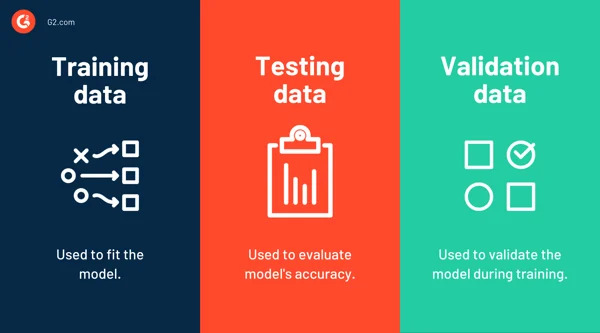
\includegraphics[width=7.5cm,height=4cm]{Pictures/ml-data/ml-datasets-type.jpg}
            \caption{Datasets: Types}
        \end{figure}
    \end{minipage}
    \hfill
    \begin{minipage}{0.45\textwidth}
        \begin{figure}[H]
            \centering
            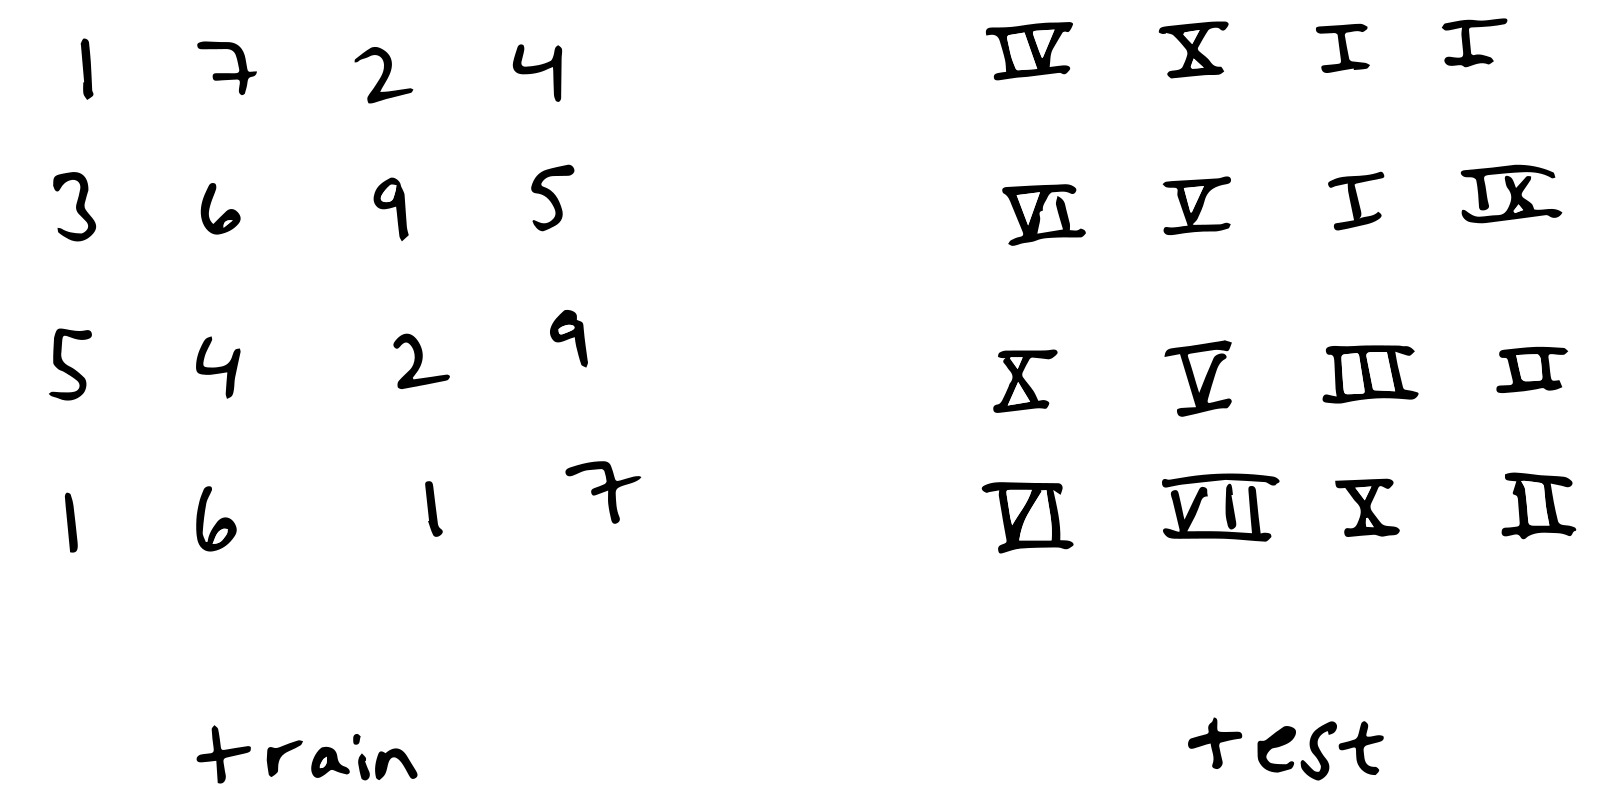
\includegraphics[width=7.5cm,height=4cm]{Pictures/ml-data/ml-data-distribution-shift.jpg}
            \caption{Distribution Shift}
        \end{figure}
    \end{minipage}
\end{table}

\subsection{Covariate shift / data shift}\label{data_shift}
Covariate shift occurs when $p(x)$ changes between train and test, but $p(y|x)$ does not. In other words, the distribution of inputs changes between train and test, but the relationship between inputs and outputs does not change.

\vspace{0.2cm}
\textbf{Examples of covariate shift:}
\begin{itemize}
    \item Self-driving car trained on the sunny streets of San Francisco and deployed in the snowy streets of Boston
    \item Speech recognition model trained on native English speakers and then deployed for all English speakers
    \item Diabetes prediction model trained on hospital data from Boston and deployed in India
\end{itemize}

\begin{table}[H]
    \begin{minipage}{0.45\textwidth}
        \begin{figure}[H]
            \centering
            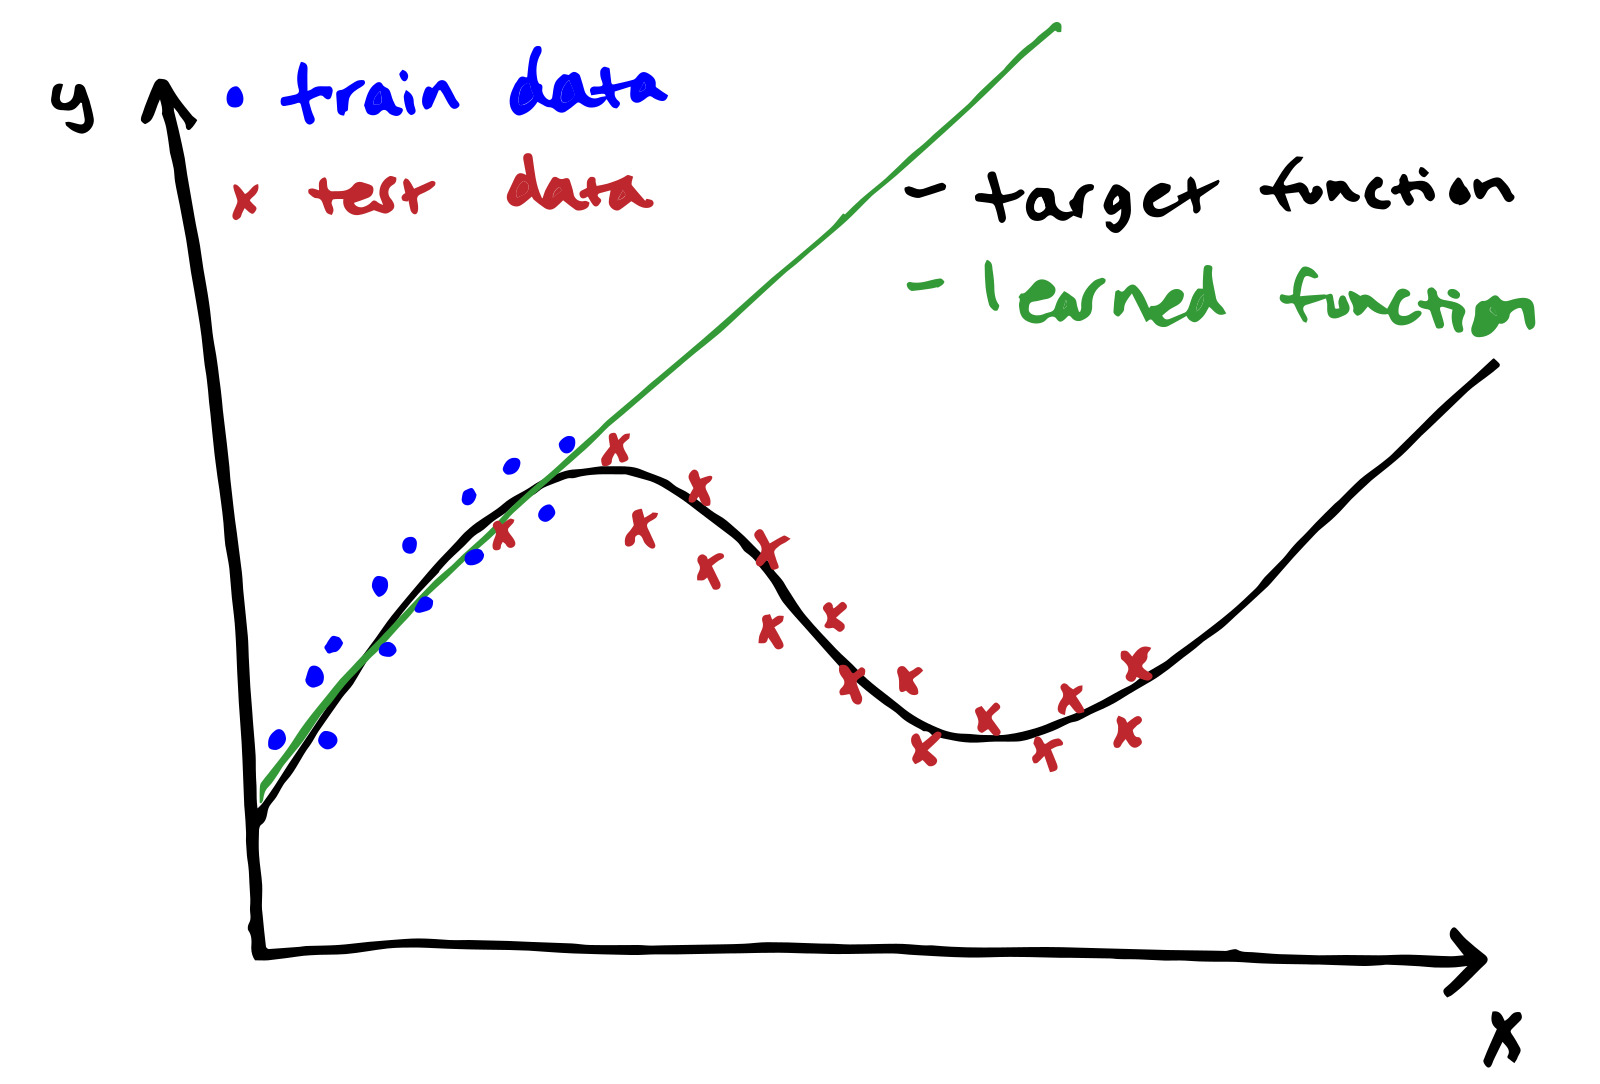
\includegraphics[width=7.5cm,height=4cm]{Pictures/ml-data/ml-data-covariate-shift.jpg}
            \caption{Distribution Shift: Covariate Shift/ Data Shift}
        \end{figure}
    \end{minipage}
    \hfill
    \begin{minipage}{0.45\textwidth}
        \begin{figure}[H]
            \centering
            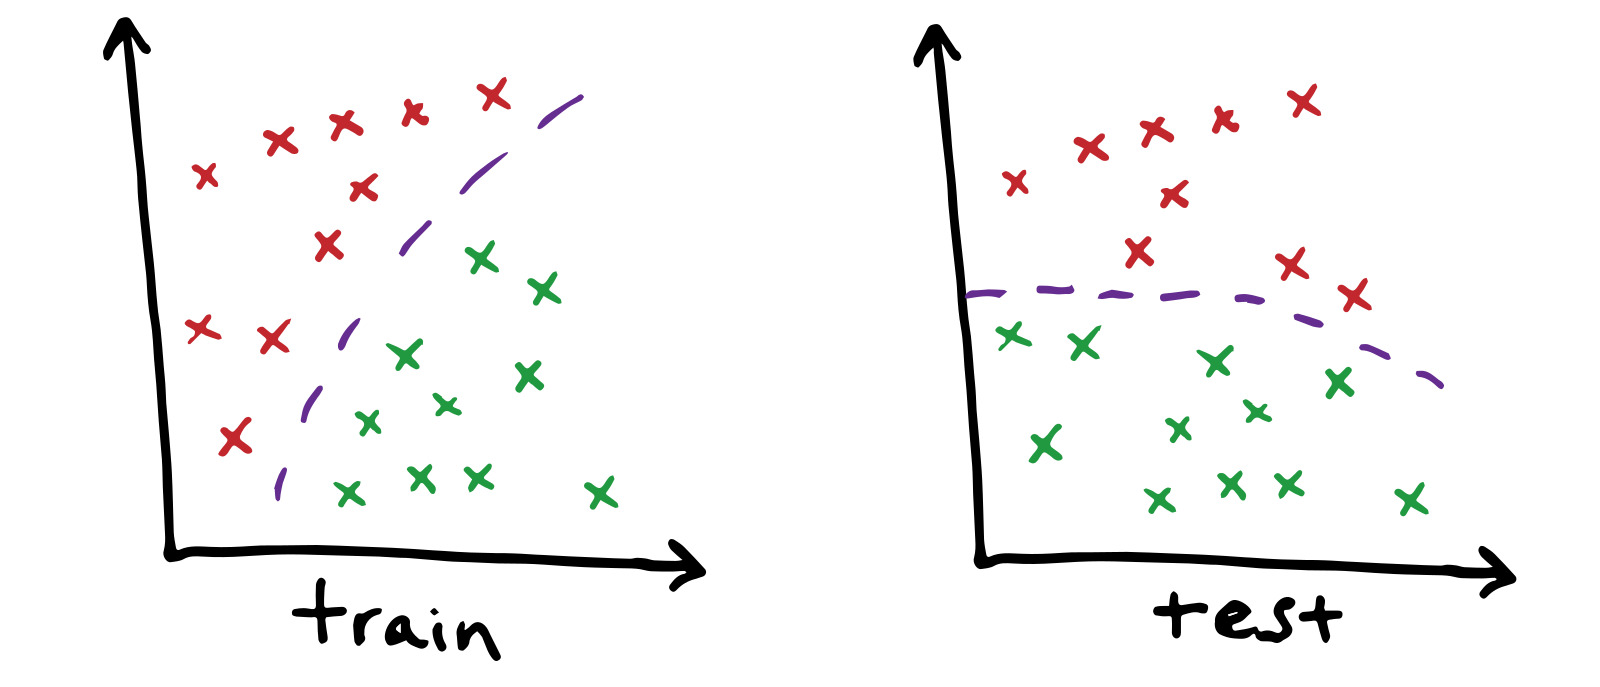
\includegraphics[width=7.5cm,height=4cm]{Pictures/ml-data/ml-data-concept-shift.jpg}
            \caption{Distribution Shift: Concept Shift}
        \end{figure}
    \end{minipage}
\end{table}

\subsection{Concept shift}\label{concept_shift}
Concept shift occurs when $p(y|x)$ changes between train and test, but $p(x)$ does not. In other words, the input distribution does not change, but the relationship between inputs and outputs does. This can be one of the most difficult types of distribution shift to detect and correct.

\vspace{0.2cm}
\textbf{Examples:}
\begin{itemize}
    \item Predicting a stock price based on company fundamentals, trained on data from 1975 and deployed in 2023.
    \item Making purchase recommendations based on web browsing behavior, trained on pre-pandemic data and deployed in March 2020.
\end{itemize}

\subsubsection{Prior probability shift / label shift}\label{label_shift}
Prior probability shift appears only in $y \to x$ problems (when we believe $y$ causes $x$). It occurs when $p(y)$ changes between train and test, but $p(x|y)$ does not. You can think of it as the converse of covariate shift.

\vspace{0.2cm}
\textbf{Examples:}
\begin{itemize}
    \item If the model is trained on a balanced dataset of 50\% spam and 50\% non-spam emails, and then it’s deployed in a real-world setting where 90\% of emails are spam, that is an example of prior probability shift.
\end{itemize}

\section{Covariate Shift (Data Shift) VS Concept Shift VS Prior Probability Shift (Label Shift) \cite{chatgpt}}


\begin{longtable}{|m{3.5cm}|m{4cm}|m{4cm}|m{4cm}|}
    \caption{Covariate Shift (Data Shift) VS Concept Shift VS Prior Probability Shift (Label Shift)} \\ \hline
    
    \textbf{Aspect} & \textbf{Covariate Shift (Data Shift)} & \textbf{Concept Shift} & \textbf{Prior Probability Shift (Label Shift)} \\ \hline
    \endfirsthead
    
    \multicolumn{4}{c}{{\bfseries \tablename\ \thetable{} -- continued from previous page}} \\ \hline
    \textbf{Aspect} & \textbf{Covariate Shift (Data Shift)} & \textbf{Concept Shift} & \textbf{Prior Probability Shift (Label Shift)} \\ \hline
    \endhead
    
    \hline \multicolumn{4}{r}{{Continued on next page}} \\ \hline
    \endfoot
    
    \hline
    \endlastfoot
    
    \textbf{Definition} & Change in the distribution of the input data (features) between training and test sets. & Change in the conditional distribution of the output given the input. & Change in the distribution of the output labels between training and test sets. \\ \hline
    
    \textbf{Cause} & Different data sources, sampling methods, or temporal changes affecting features. & Changes in the underlying relationship between features and labels, often due to evolving contexts or environments. & Variations in the frequency or proportion of different labels in the dataset over time. \\ \hline

    \textbf{Effect} & Model performance degradation due to misaligned feature distributions. & Model predictions become inaccurate because the learned relationships are no longer valid. & Bias in predicted label distribution if not accounted for, leading to misclassification. \\ \hline

    \textbf{Detection} & Comparing feature distributions (e.g., using statistical tests like KS test, histograms). & Analyzing the performance metrics over time or checking for changes in decision boundaries. & Comparing label distributions (e.g., using chi-square tests) or through domain knowledge. \\ \hline

    \textbf{Adjustment Techniques} & Reweighting samples, domain adaptation methods, or using robust models. & Regular retraining with updated data, transfer learning, or domain adaptation techniques. & Adjusting model outputs using methods like importance weighting, resampling, or calibration. \\ \hline

    \textbf{Example} & A retail model trained on summer sales data might perform poorly in winter due to changes in purchasing behavior. & A spam detection model might become less effective if spammers change tactics and the nature of spam emails evolves. & A medical diagnosis model might require adjustment if the prevalence of certain diseases changes in the population. \\ \hline

    \textbf{Relevance in Real-world Applications} & High when dealing with non-stationary environments or merging datasets from different sources. & High in dynamic environments where the relationship between input features and output labels can evolve. & High in situations with shifting class distributions, like seasonal changes or demographic shifts. \\ \hline

\end{longtable}


















